\documentclass[a4paper,twoside]{article}
\usepackage{blindtext}  
\usepackage{geometry}

% Chinese support
\usepackage[UTF8, scheme = plain]{ctex}

% Page margin layout
\geometry{left=2.3cm,right=2cm,top=2.5cm,bottom=2.0cm}


\usepackage{listings}
\usepackage{xcolor}
\usepackage{geometry}
\usepackage{amsmath}
\usepackage{float}
\usepackage{hyperref}

\usepackage{graphics}
\usepackage{graphicx}
\usepackage{subfigure}
\usepackage{epsfig}
\usepackage{float}

\usepackage{algorithm}
\usepackage[noend]{algpseudocode}

\usepackage{booktabs}
\usepackage{threeparttable}
\usepackage{longtable}
\usepackage{listings}
\usepackage{tikz}

% cite package, to clean up citations in the main text. Do not remove.
\usepackage{cite}

\usepackage{color,xcolor}

%% The amssymb package provides various useful mathematical symbols
\usepackage{amssymb}
%% The amsthm package provides extended theorem environments
\usepackage{amsthm}
\usepackage{amsfonts}
\usepackage{enumerate}
\usepackage{enumitem}
\usepackage{listings}

\usepackage{indentfirst}
\setlength{\parindent}{2em} % Make two letter space in the first paragraph
\usepackage{setspace}
\linespread{1.5} % Line spacing setting
\usepackage{siunitx}
\setlength{\parskip}{0.5em} % Paragraph spacing setting

% \usepackage[contents =22920202204622, scale = 10, color = black, angle = 50, opacity = .10]{background}

\renewcommand{\figurename}{图}
\renewcommand{\lstlistingname}{代码} 
\renewcommand{\tablename}{表格}
\renewcommand{\contentsname}{目录}
\floatname{algorithm}{算法}

\graphicspath{ {images/} }

%%%%%%%%%%%%%
\newcommand{\StudentNumber}{22920202204622}  % Fill your student number here
\newcommand{\StudentName}{熊恪峥}  % Replace your name here
\newcommand{\PaperTitle}{实验(二)\ \ 实现FFT}  % Change your paper title here
\newcommand{\PaperType}{计算方法(A)} % Replace the type of your report here
\newcommand{\Date}{2022年4月5日}
\newcommand{\College}{信息学院}
\newcommand{\CourseName}{计算方法(A)}
%%%%%%%%%%%%%

%% Page header and footer setting
\usepackage{fancyhdr}
\usepackage{lastpage}
\pagestyle{fancy}
\fancyhf{}
% This requires the document to be twoside
\fancyhead[LO]{\texttt{\StudentName }}
\fancyhead[LE]{\texttt{\StudentNumber}}
\fancyhead[C]{\texttt{\PaperTitle }}
\fancyhead[R]{\texttt{第{\thepage}页,共\pageref*{LastPage}页}}


\title{\PaperTitle}
\author{\StudentName}
\date{\Date}

\lstset{
	basicstyle          =   \sffamily,          % 基本代码风格
	keywordstyle        =   \bfseries,          % 关键字风格
	commentstyle        =   \rmfamily\itshape,  % 注释的风格,斜体
	stringstyle         =   \ttfamily,  % 字符串风格
	flexiblecolumns,                % 别问为什么,加上这个
	numbers             =   left,   % 行号的位置在左边
	showspaces          =   false,  % 是否显示空格,显示了有点乱,所以不现实了
	numberstyle         =   \zihao{-5}\ttfamily,    % 行号的样式,小五号,tt等宽字体
	showstringspaces    =   false,
	captionpos          =   t,      % 这段代码的名字所呈现的位置,t指的是top上面
	frame               =   lrtb,   % 显示边框
}

\lstdefinestyle{PythonStyle}{
	language        =   Python, % 语言选Python
	basicstyle      =   \zihao{-5}\ttfamily,
	numberstyle     =   \zihao{-5}\ttfamily,
	keywordstyle    =   \color{blue},
	keywordstyle    =   [2] \color{teal},
	stringstyle     =   \color{magenta},
	commentstyle    =   \color{red}\ttfamily,
	breaklines      =   true,   % 自动换行,建议不要写太长的行
	columns         =   fixed,  % 如果不加这一句,字间距就不固定,很丑,必须加
	basewidth       =   0.5em,
}

\algnewcommand\algorithmicinput{\textbf{Input:}}
\algnewcommand\algorithmicoutput{\textbf{Output:}}
\algnewcommand\Input{\item[\algorithmicinput]}%
\algnewcommand\Output{\item[\algorithmicoutput]}%

\usetikzlibrary{positioning, shapes.geometric}

\begin{document}
	
%%%%%%%%%%%%%%%%%%%%%%%%%%%%%%%%%%%%%%%%%%%%
\makeatletter % change default title style
\renewcommand*\maketitle{%
	\begin{center} 
		\bfseries  % title 
		{\LARGE \@title \par}  % LARGE typesetting
		\vskip 1em  %  margin 1em
		{\global\let\author\@empty}  % no author information
		{\global\let\date\@empty}  % no date
		\thispagestyle{empty}   %  empty page style
	\end{center}%
	\setcounter{footnote}{0}%
}
\makeatother
%%%%%%%%%%%%%%%%%%%%%%%%%%%%%%%%%%%%%%%%%%%%
	
	
\thispagestyle{empty}

\vspace*{1cm}

\begin{figure}[h]
	\centering
	
\includegraphics[width=4.0cm]{logo.png}
\end{figure}

\vspace*{1cm}

\begin{center}
	\Huge{\textbf{\PaperType}}
	
	\Large{\PaperTitle}
\end{center}

\vspace*{1cm}

\begin{table}[h]
	\centering	
	\begin{Large}
		\renewcommand{\arraystretch}{1.5}
		\begin{tabular}{p{3cm} p{5cm}<{\centering}}
			姓\qquad 名 & \StudentName  \\
			\hline
			学\qquad号 & \StudentNumber \\
			\hline
			日\qquad期 & \Date  \\
			\hline
			学\qquad院 & \College  \\
			\hline
			课程名称 & \CourseName  \\
			\hline
		\end{tabular}
	\end{Large}
\end{table}

\newpage

\title{
	\Large{\textcolor{black}{\PaperTitle}}
}
	
	
\maketitle
	
\tableofcontents
 
\newpage
\setcounter{page}{1}

\begin{spacing}{1.2}

\section{原理}

傅里叶变换将信号的时域采样变换到频域,这样就可以对信号进行操作,比如加噪声、滤波、抽样等。通过傅里叶变换,可以在图像的频域增加信息,用于追溯信息泄露等工作。
快速傅里叶变换(FFT)是一种用于快速计算离散傅里叶变换(DFT)的算法。它借助了$\omega=e^{-\frac{2\pi i}{N}}$的对称性~\eqref{eqn:sym}

\begin{equation}
	\label{eqn:sym}
	\omega_N^{jk+N/2}=-\omega_N^{jk}
\end{equation}
可以得到~\eqref{eqn:calc}和~\eqref{eqn:calc2}
\begin{gather}
	\label{eqn:calc}
	c_{2j}=\sum_{k=0}^{N/2-1}\left(x_k+x_{N/2+k}\right)w_{N/2}^{jk}, \\
	\label{eqn:calc2}
	c_{2j+1}=\sum_{k=0}^{N/2-1}\left(x_k-x_{N/2+k}\right)w_{N}^{k}w_{N/2}^{jk}
\end{gather}
因此可以由\nameref{sec:app}中的代码~\ref{code:fft_rec}递归地计算FFT,它的时间复杂度是$\mathcal{O}(N\log N)$。这叫做Cooley-Tukey算法。
其中$padding$函数可以用来在输入点数不是2的倍数时填充0,以使得输入点数变成2的倍数。它使用了位运算技巧来获取离~$x$~长度最接近的2的幂。

\section{结果}

对$y=x^2\cdot\cos x$在$[-\pi,\pi]$上逼近,等距离取$16$个点,逼近结果和函数$y=x^2\cdot\cos x$如图~\ref{fig:result}。
可见FFT逼近效果较好,误差主要出现在区间两端点附近。其余部分与函数较为相近。进一步增加点数可以使得逼近效果更佳。

\begin{figure}[htbp]
	\begin{minipage}[t]{0.48\linewidth}
		\centering
		\label{fig:result}
		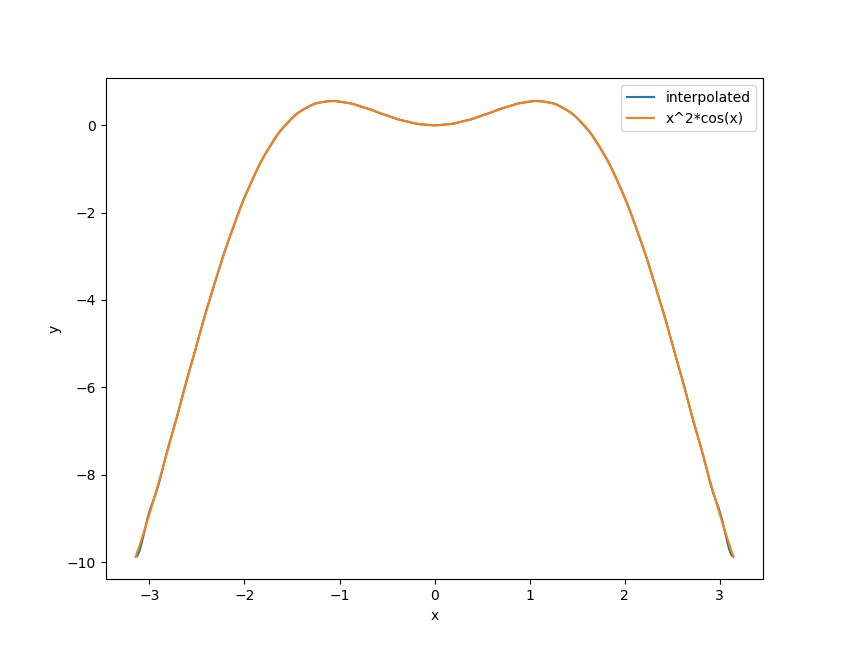
\includegraphics[width=\linewidth]{result.png}
		\caption{逼近结果和$y=x^2\cdot\cos x$}
	\end{minipage}
	\begin{minipage}[t]{0.48\linewidth}
		\centering
		\label{fig:freqs}
		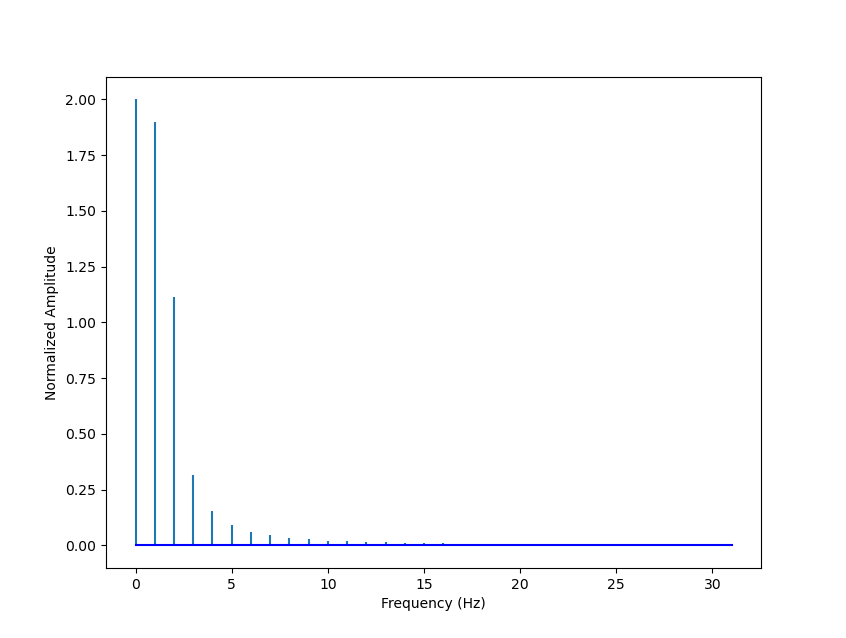
\includegraphics[width=\linewidth]{freqs.png}
		\caption{逼近结果的频率和幅度}
	\end{minipage}
\end{figure}

FFT使用三角函数的组合对函数进行逼近,各三角函数的频率和幅值如图~\ref{fig:freqs}。图示幅值经过\eqref{eqn:normalize_amp}
的归一化处理来减少幅值绝对值之间的差,便于展示。

\begin{equation}
	\label{eqn:normalize_amp}
	A_{normalized}=\frac{|A|}{N/2}
\end{equation}

实践表明增加取点个数可以很好地提高FFT逼近函数的效果。

\begin{figure}[H]
	\centering
	\label{fig:result2}
	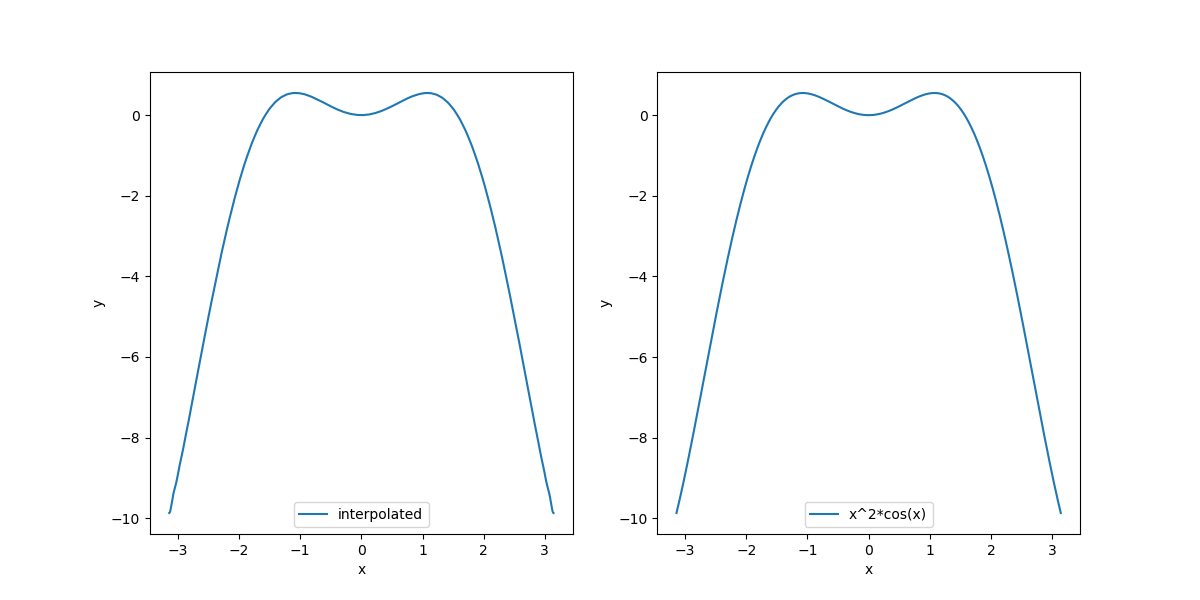
\includegraphics[width=0.8\linewidth]{result_morepoints.png}
	\caption{取点数$N=64$逼近结果和$y=x^2\cdot\cos x$}
\end{figure}

如图~\ref{fig:result2}取$N=64$,可见逼近曲线光滑、与函数曲线较为相近。进一步提高了逼近效果。

将这些三角函数和函数$y=x^2\cdot \cos x$画在同意坐标系中如图,$y=x^2\cdot \cos x$人为画在$f=-2.5$处,可以直观地
展现出\emph{FFT将函数分解为频率不同、幅值不同的三角函数的作用}。

\begin{figure}[H]
	\centering 
	\subfigure[视角1]{ 
	  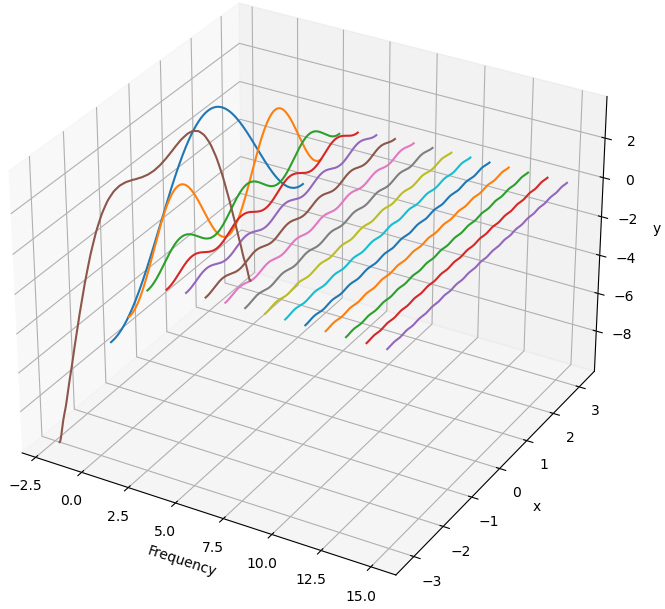
\includegraphics[width=0.48\textwidth]{freq3d_1.png} 
	} 
	~
	\subfigure[视角2]{ 
	  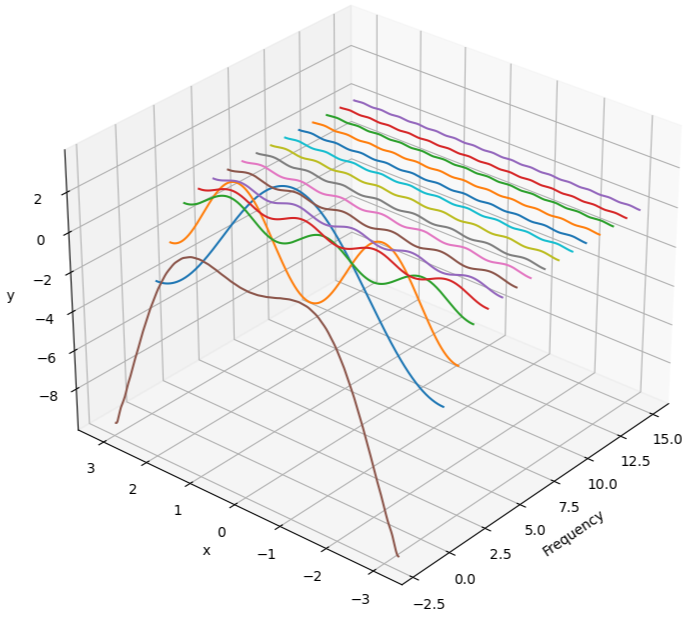
\includegraphics[width=0.48\textwidth]{freq3d_2.png} 
	} 
	\caption{FFT结果的各频域分量} 
	\label{fig:freq3d}
\end{figure}

\clearpage

\appendix
\section{附录A:实现代码}
\label{sec:app}

\begin{lstlisting}[language=Python,numbers=left,style=PythonStyle,label={code:fft_rec},caption=FFT实现]
def padding(x: np.ndarray) -> np.ndarray:
    n: int = x.shape[0]

    if (n & (n - 1)) == 0:
        return x

    n -= 1
    n |= n >> 1
    n |= n >> 2
    n |= n >> 4
    n |= n >> 8
    n |= n >> 16
    n += 1

    return np.pad(x, (0, n - x.shape[0]))

def fft(x: np.ndarray) -> np.ndarray:
    x = padding(x)
    N: Final[float] = x.shape[0]

    if N == 1:
        return x
    else:
        even = fft(x[::2])
        odd = fft(x[1::2])

        fact = np.exp(-2j * np.pi * np.arange(N) / N)

        return np.hstack((even + fact[:int(N / 2)] * odd, even + fact[int(N / 2):] * odd))


\end{lstlisting}

\end{spacing}

\end{document}